Для получения информации об атомном облаке в МОЛ использовалась схема изображенная на рис. \ref{fig:exp_photo}. 

\begin{figure}[h]
    \centering
    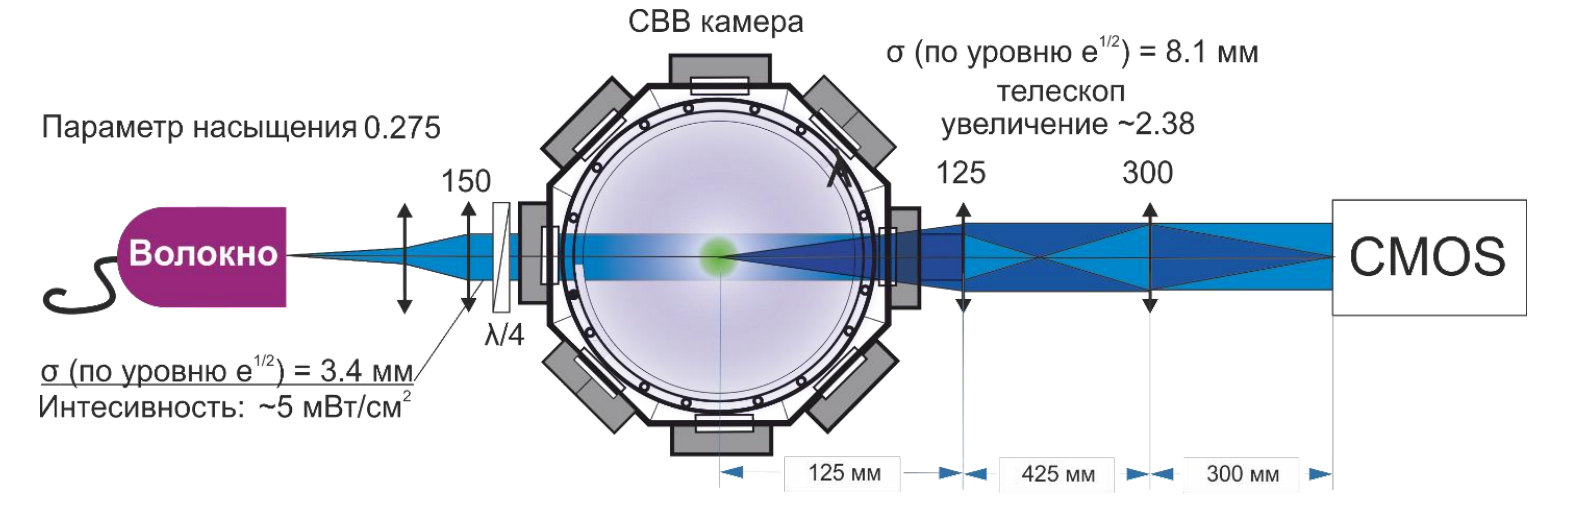
\includegraphics[width=0.9\textwidth]{figs/detect.png}
    \caption{Схема детектирования из \cite{vlad}}
    \label{fig:exp_photo}
\end{figure}


В соответствии с законом Бугера-Ламберта-Бера интенсивность резонансного лазерного пучка после прохождения через облако может быть найдена в виде
\begin{equation}
    \frac{d I}{d z} = - \sigma n I,
    \hspace{10 mm} 
    \sigma = \frac{\sigma_0}{1+I/I_s + 4 (\delta/\Gamma)^2},
\end{equation}
где $I_s$ -- интенсивность насыщения, $\delta$ -- отстройка от резонанса, $n$ -- концентрация атомов в ловушке, $\sigma_0 = 3 \lambda^2 / 2\pi$ -- резонансное сечение поглощения атомом одиночного фотона, $\lambda$ -- длина волны света. Для измерения параметров атомного облага с помощью CMOS камеры делается фотография лазерного пучка без атомов, что даёт распределение интенсивности $\subt{I}{D}$, затем делается фотография тени от атомов $I_0$, и по ним вычисляется распределение атомов $\sub{f}{exp}(x, y)$ (рис. \ref{fig:fitmot}):
\begin{equation}
    \sub{f}{exp} = \ln\left(\frac{\subt{I}{D}}{I_0}\right) + \frac{\subt{I}{D} - I_0}{I_s} = \sigma_0 \int n(x, y, z) \d z.
\end{equation}





\begin{figure}[h]
    \centering
    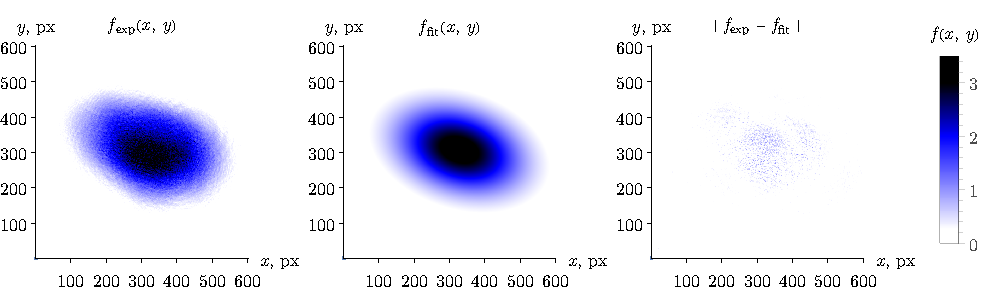
\includegraphics{figs/fit_mot.pdf}
    \caption{...}
    \label{fig:fitmot}
\end{figure}



